\documentclass[12pt]{article}

% ----- Preamble
\usepackage[utf8]{inputenc} % police encodee en latin1=iso8859-1=Windows Latin 1 %
\usepackage[french]{babel} % police fr %
\usepackage{hyperref} % pour les references %
\usepackage{amsmath} % pour les formules de maths %
\usepackage{amssymb} % pour les symboles maths %
\usepackage{amsthm} % pour la mise en forme des theoremes %
\usepackage{aeguill} % pour les guillemets et accents francais %
\usepackage{listings} % pour les listings de code %
\usepackage{helvet} % police helvetica %
\usepackage{graphicx}
\usepackage{centernot}
\usepackage{dsfont}
% modification des dimensions de la page et de son centrage %
\topmargin 0.0cm
\oddsidemargin 0.2cm
\textwidth 16cm 
\textheight 21cm
\footskip 0.0cm

\title{Traitement d'Image et du Signal - TP3}
\author{Laurent Cetinsoy, Karim Kouki, Aris Tritas }
\date{\today}

\begin{document}
\maketitle

\section{Rotation d'image}

\subsection{Introduction} 

Pour chaque point $(x, y)$ de l'image originale nous souhaitons utiliser la TFD pour calculer le point $(x', y')$ résultant d'une rotation d'angle  $\theta \in {[0, 2\pi]}$. On peut définir la rotation par la matrice \textbf{M} ci-dessous:
$$\begin{pmatrix}
x' \\ y'
\end{pmatrix}=
\begin{pmatrix}
\cos \theta & -\sin \theta \\
\sin \theta & \cos \theta
\end{pmatrix}
\begin{pmatrix}
x \\ y
\end{pmatrix}=\textbf{M}
\begin{pmatrix}
x \\ y
\end{pmatrix}
$$
où \textbf{M} peut être ré-exprimée comme suit (e.g. \cite{paeth86}):
$$M =
\begin{pmatrix}
1 & -\tan \frac{\theta}{2} \\
0 & 1
\end{pmatrix}
\begin{pmatrix}
1 & 0 \\
\sin \theta & 1
\end{pmatrix}
\begin{pmatrix}
1 & -\tan \frac{\theta }{2}\\
0 & 1
\end{pmatrix}
$$
L'idée de \cite{unser95} \cite{larkin97} est d'utiliser trois convolutions linéaires (et donc séparables) qui distordent l'image successivement selon les axes $x$, $y$ et $x$. 
Chacune s'écrit comme une translation dans le domaine de Fourier. La distortion $u_{dx}(x, y) = u(x + ay, y)$ pour l'axe $x$ (où $a$ contrôle l'angle) s'exprime par l'opérateur suivant:
$$ D_x(\xi) = \mathcal{F}\{u_d(x, y)\} = \mathcal{F}\{u(x, y)\} e^{-2 i \pi \xi a y}$$


Si l'on répête cette opération pour $y$ et encore une fois pour $x$ l'on retrouve le signal réel pivoté. L'image originale est insérée dans une image plus grande afin de ne pas être tronquée. \newline

\subsection{Experimentations}

Les expériences suivantes ont été menées : 
\begin{itemize}
\item Rotations d'images avec des images bruitées et non bruitées.
\item N rotations d'angle $\frac{2\pi}{N}$ successives d'une même image. 
\end{itemize}

\subsubsection{Rotations simples}


L'algorithme a été testé pour plusieurs valeurs d'angles sur des images bruitées ou non. Dans le cas général il donne fonctionne correctement en conservant la qualité de l'image initiale. Néanmoins pour $\theta = \frac{2\pi}{3}$ les bords de l'image se détachent. Il n'a pas été possible de trouver la cause du problème. 
pour $\theta = \pi$ l'algorithme ne fonctionne pas comme cela a été annoncé dans le cours. 

\begin{figure}[h]
	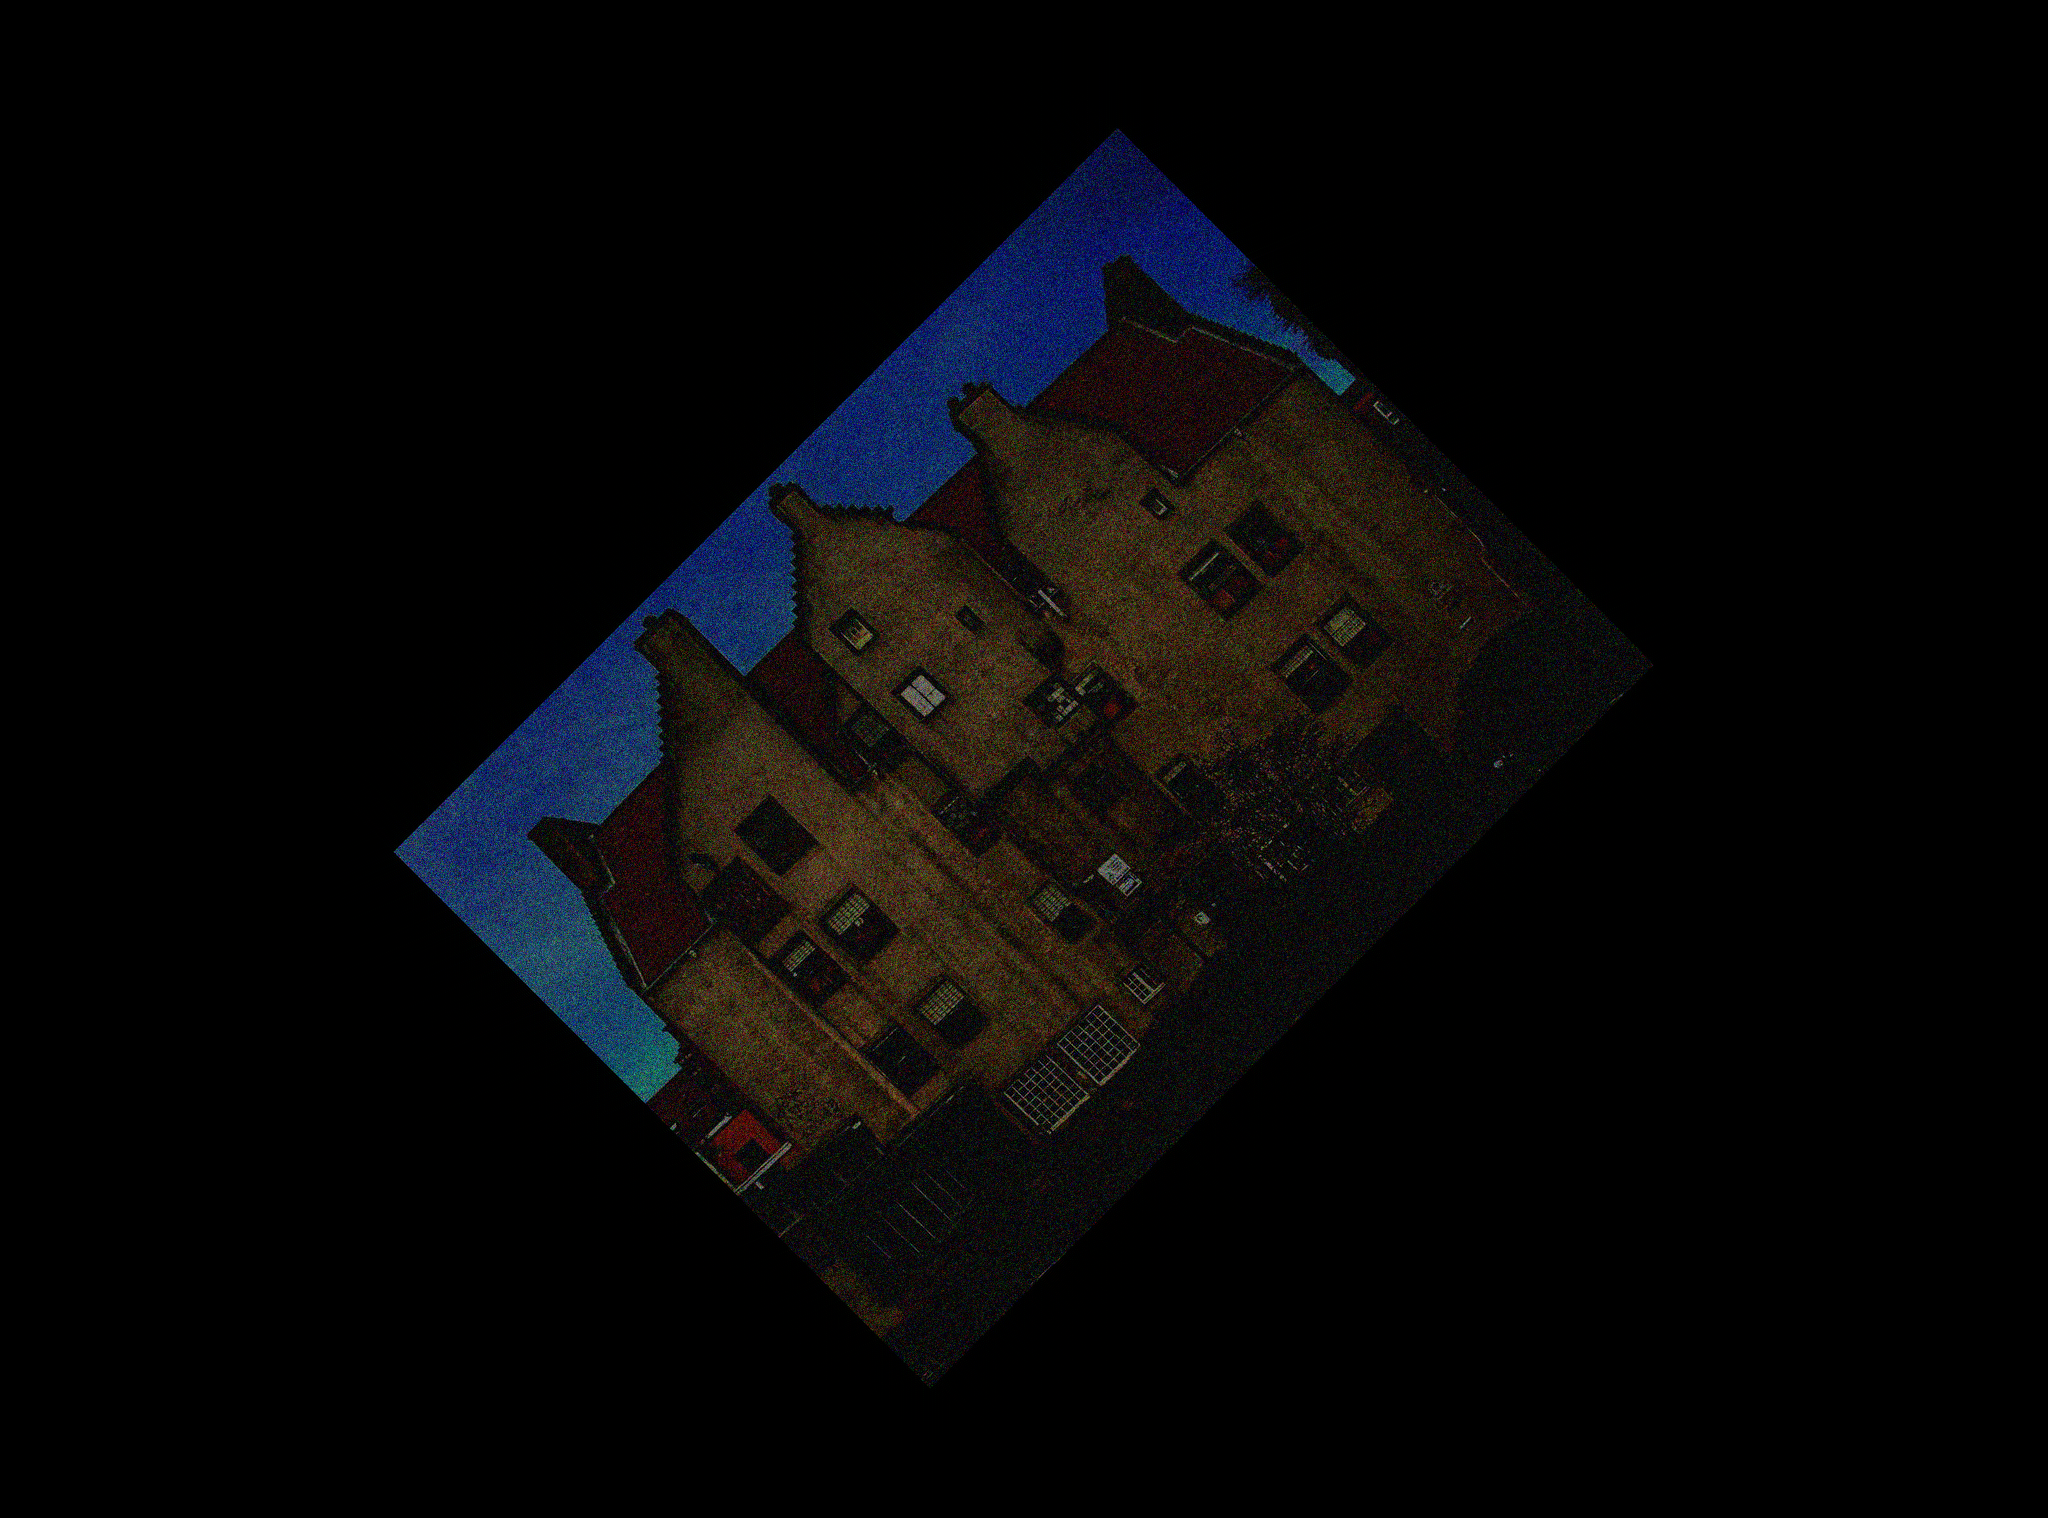
\includegraphics[width=0.25\textwidth]{castle_bruite_2pi_over_8.png}
	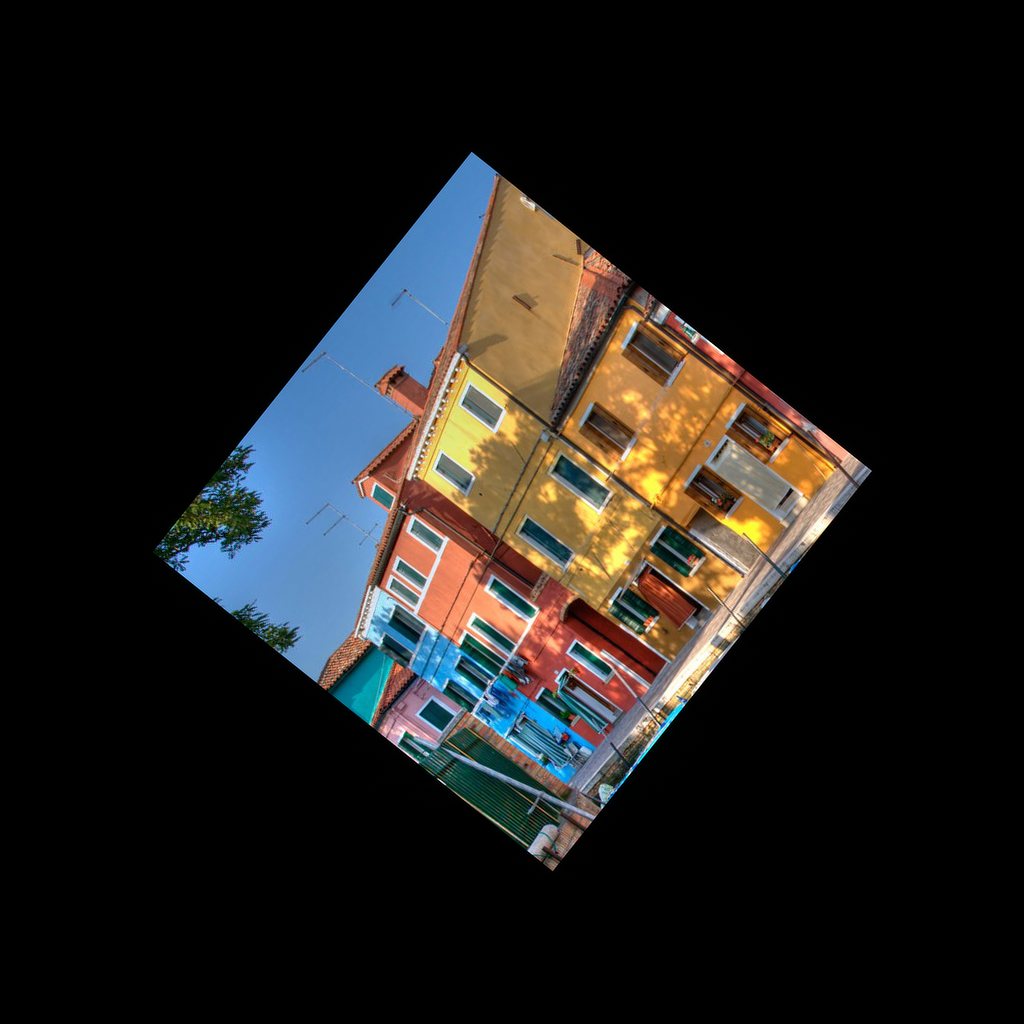
\includegraphics[width=0.20\textwidth]{house_rotation_2pi_over_7.png}
    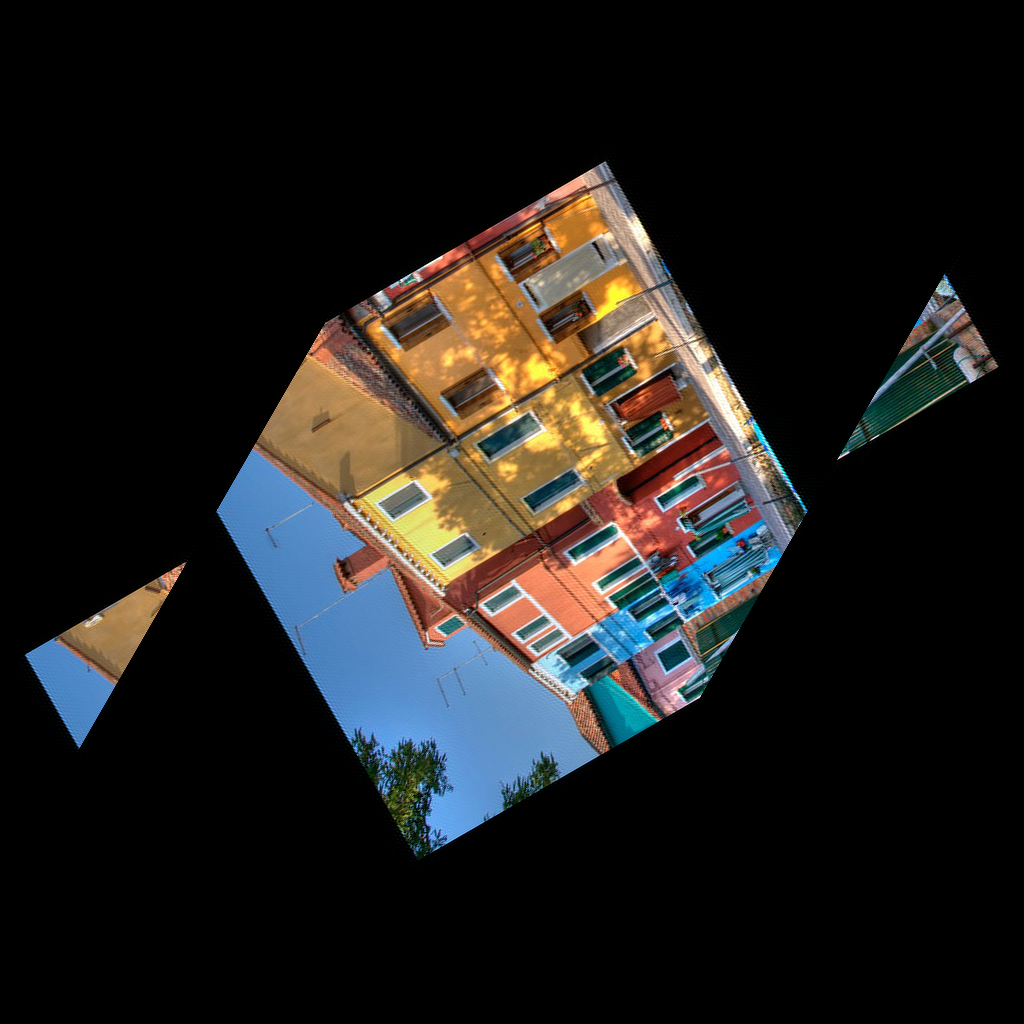
\includegraphics[width=0.20\textwidth]{house_rotation_2pi_over_3.png}
    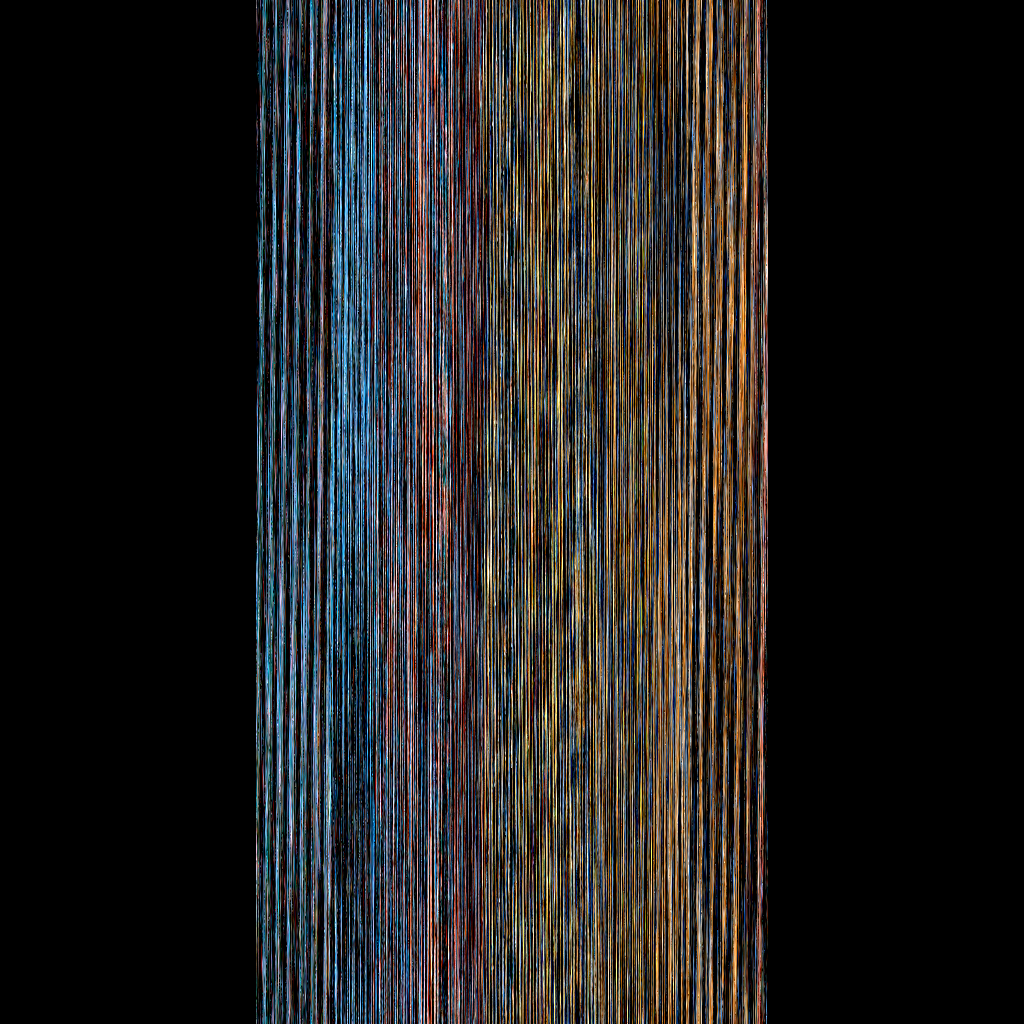
\includegraphics[width=0.20\textwidth]{house_rotation_pi.png}
    \caption{De gauche à droite : $\theta = \frac{2\pi}{8}$, $\theta = \frac{2\pi}{7}$, $\theta = \frac{2\pi}{3}$, $\theta = \pi$. }
    
\end{figure}



\subsubsection{Rotation multiple d'une image}

Une succession de rotation d'angle $\theta = \frac{2\pi}{N}$ a été effectuée sur une image afin de pouvoir comparer l'image originale et l'image après N rotations. 

\begin{figure}[h]
	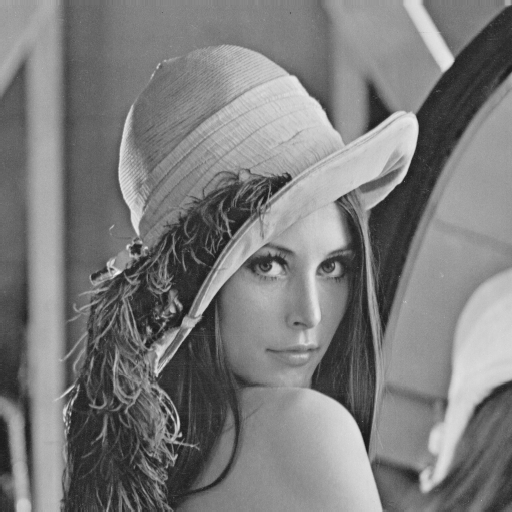
\includegraphics[width=0.15\textwidth]{lena.png}
	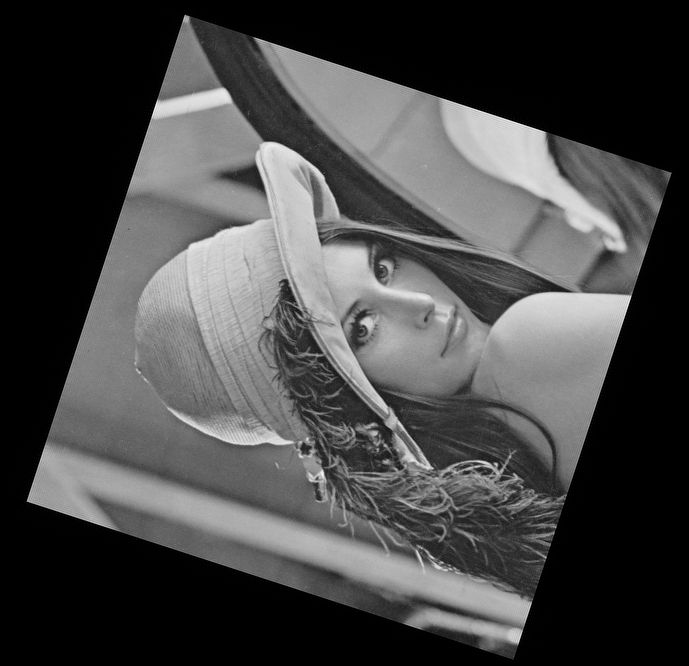
\includegraphics[width=0.15\textwidth]{rotation_2pi_1.png}
	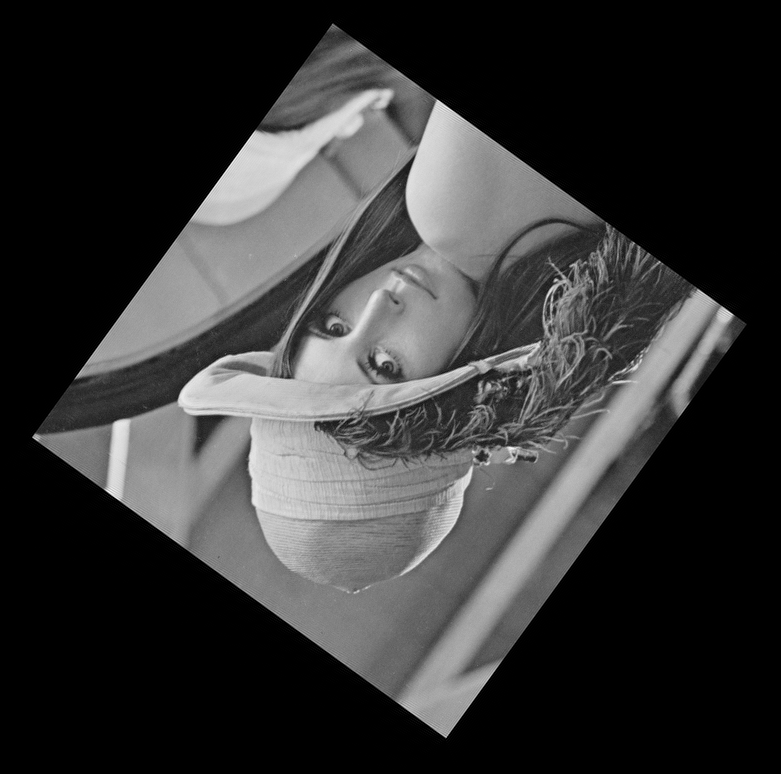
\includegraphics[width=0.15\textwidth]{rotation_2pi_2.png}
	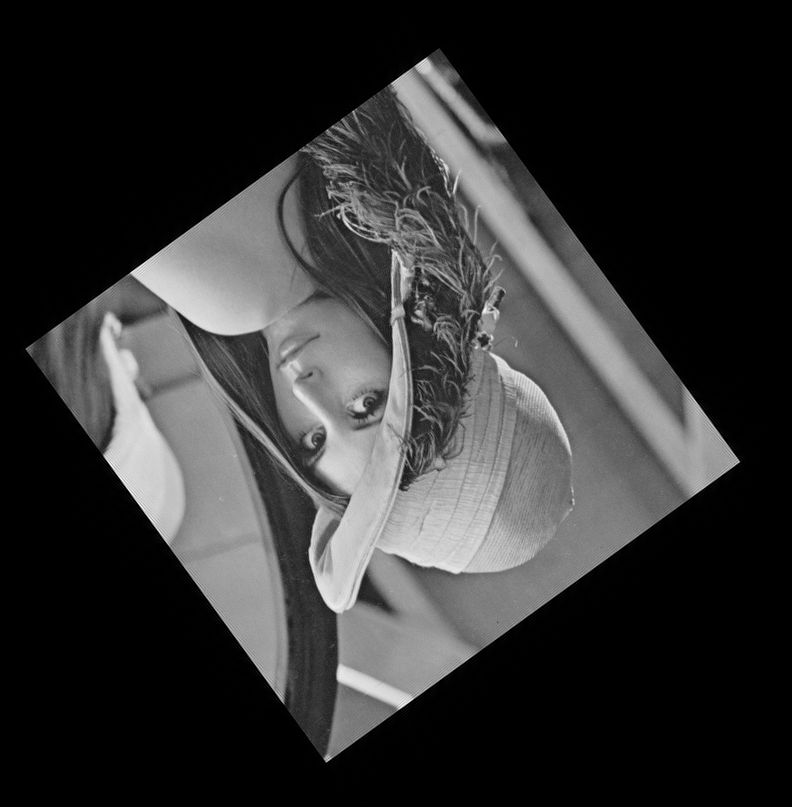
\includegraphics[width=0.15\textwidth]{rotation_2pi_3.png}
	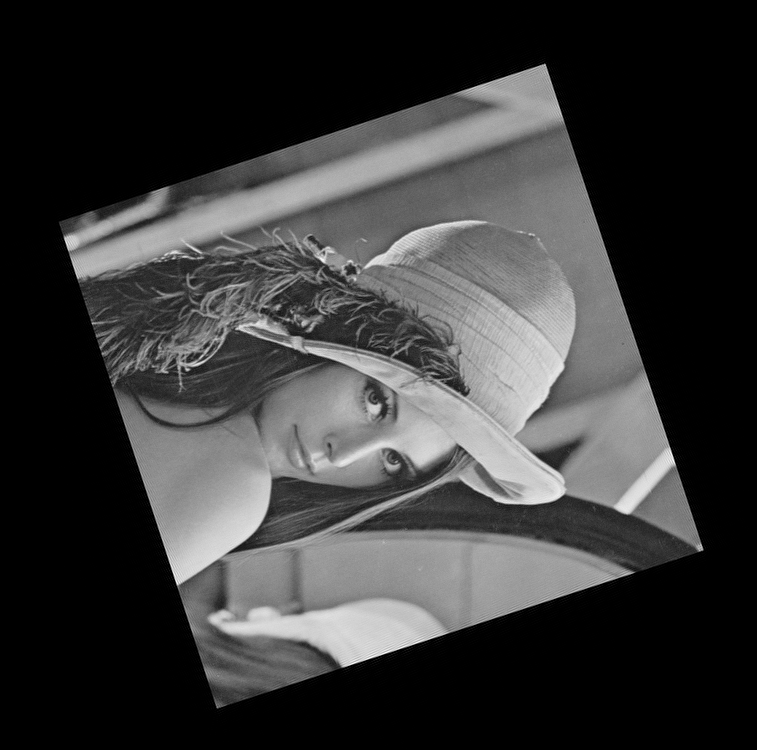
\includegraphics[width=0.15\textwidth]{rotation_2pi_4.png}
	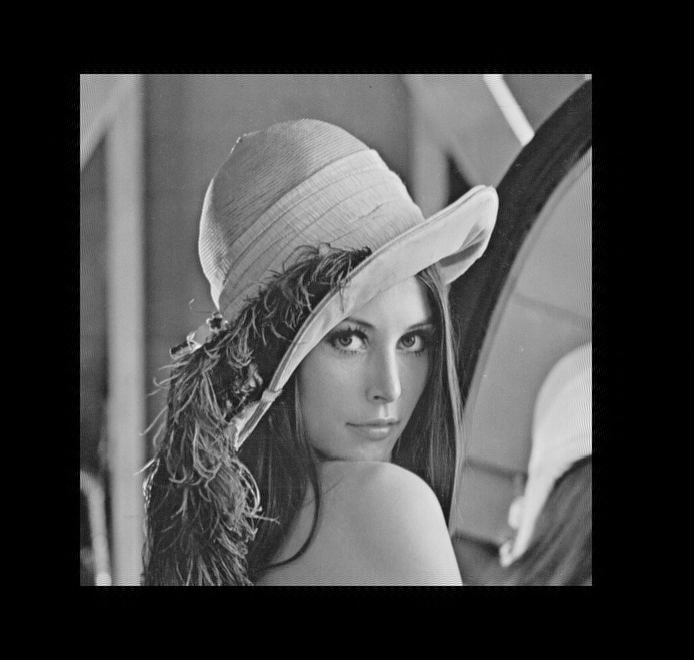
\includegraphics[width=0.15\textwidth]{rotation_2pi_5.png}
  \caption{A gauche l'image originale, à droite les rotations successives d'angle $\theta = \frac{2\pi}{5}$.}
\end{figure}

On constate que l'image a une qualité sembable à celle de l'originale. 

\subsection{Discussion}

L'implémentation de l'algorithme souffre des limites suivantes : 
\begin{itemize}

\item Il ne gère pas les angles $\frac{k\pi}{2}$ où serait en fait possible de se passer de la transformée de fourier et éviter le problème de rotation de $theta =  k\pi$.
\item Le zero-padding utilisé  inclut l'image originale dans une image aggrandie par un facteur constant. Il y a donc bien plus de zero que nécessaire : il serait avantageux de raboter l'image afin que la taille de l'image soit définie par les coin de l'image originale. En effet dans l'expérience de rotation successive, la taille de l'image à l'étape i est zoom$^i$ ce qui rend l'expérience impossible à pratiquer pour de grandes valeurs de $N$.
\item Le problème de l'angle de $\frac{k\pi}{3}$ où deux des coins de l'image se détachent.

\end{itemize}

\section{Exercices}

Notons le signal d'entrée $e(t)$ et le signal de sortie $s(t)$.


\textbf{Définition} Système linéaire: pour $\alpha_1, \alpha_2 \in \mathbb{R}$\newline
Si $e_1(t) \rightarrow s_1(t)$ et $e_2(t) \rightarrow s_2(t)$, alors $\alpha_1 e_1(t) + \alpha_2 e_2(t) \rightarrow \alpha_1 s_1(t) + \alpha_2 s_2(t)$

\textbf{Définition} Système invariant: pour $\tau \in \mathbb{R}$ \newline
Si $e(t) \rightarrow s(t)$ alors $e(t-\tau) \rightarrow s(t-\tau)$, $\tau$ étant une constante de décalalage.

\textbf{Définition} Produit de convolution de deux suites $u_n$ et $h_n$: \newline
$$ (u \otimes h)(n) = \sum_{k \in \mathbb{Z}} u_{n-k}h_k $$

\textbf{Définition} Réponse impulsionnelle: \newline
La sortie d'un système linéaire invariant est égale au produit de convolution de l'entrée par la réponse impulsionnelle $h, \;\;e(t) \longrightarrow s(t) = (e \otimes h)(t)$


\subsection*{Exercice 1}
Pour les questions (1)-(4), l'entrée est la suite $u_n$ et la sortie la suite $v_n$ pour $n \in \mathbb{Z}$. \newline
Pour les questions (5) et (6) l'entrée est une fonction $f \in \mathrm{L}^1 \cap \mathrm{L}^2$ définie sur $\mathbb{R}$ et la sortie est une fonction $g(x): \; \mathbb{R} \rightarrow \mathbb{R}$
\begin{enumerate}
\item $v_n = u_n - u_{n-1} + 3u_{n+1}$: \newline
La relation est une somme de termes décalés et comporte des produits avec des scalaires, elle est donc linéaire. $\alpha(u_n - u_{n-1} + 3u_{n+1}) \rightarrow \alpha v_n$ \newline
La relation est invariante car $u_{n-\tau} - u_{n-1-\tau} + 3u_{n+1-\tau} \rightarrow v_{n-\tau}$ \newline
La réponse impulsionnelle peut être donnée par identification des termes de la somme du produit de convolution: $h_{-1} = 3, h_0 = 1, h_1 = -1$
\item $v_n = u_{2n}$: \newline
La relation impulsionnelle est un sous échantillonnage qui est linéaire. En effet $\alpha u_{2n} \rightarrow \alpha v_n$. De plus, sous-échantillonner la somme de deux signaux revient à sommer les sous-échantillons de ces signaux.
La relation est non-invariante par translation car $u_{2n-\tau} \centernot\longrightarrow v_{n-\tau} (=u_{2(n-\tau)})$
\item $v_n = \max(u_n, u_{n-1}, u_{n+1})$: \newline
L'opérateur max n'est pas linéaire. Considérons les suites $u_n$ et $u_n'$ définies par: \newline
\begin{itemize}
\item $u_k = u_k' = 0 \;\forall k \in \mathbb{Z} \setminus \{0, 1, 2\}$
\item $u_0 = -1, u_1 = -1, u_2 = -10 $
\item $u_0' = -1, u_1' = 1, u_2' = 10 $
\end{itemize}
Il s'ensuit: 
\begin{equation*}
\begin{split}
 v_n + v_n' &= \max(u_0, u_1, u_2) + \max(u_0', u_1', u_2') \\
			&= \max(-1, -1, -10) + \max(-1, 1, 10) \\
			&= 9 \\
			&\neq \max(-1-1, -1+1, -10 + 10) = 1
\end{split}
\end{equation*}
\item $v_n = u_{n-1}$: \newline
La réponse est linéaire car $\alpha u_{n-1} \rightarrow \alpha v_n$ et invariante par translation \newline car $u_{n-1-\tau} \rightarrow v_{n-\tau}$ \newline
De même que pour la question 1, la réponse impulsionnelle peut être donnée par identification du terme non-nul du produit de convolution: $h_{-1} = 1$
\item $g(x) = \int_{x-\frac{1}{2}}^{x+\frac{1}{2}} f(t) \,\mathrm{d}t$: \newline
La relation est linéaire par linéarité de l'intégration: $$\int_{x-\frac{1}{2}}^{x+\frac{1}{2}} f_1(t) + f_2(t) \,\mathrm{d}t = \int_{x-\frac{1}{2}}^{x+\frac{1}{2}} f_1(t) \,\mathrm{d}t+ \int_{x-\frac{1}{2}}^{x+\frac{1}{2}} f_2(t) \,\mathrm{d}t$$ \newline
La relation est invariante par translation: soit l'entrée $f(t-\tau)$, \newline en posant $t' = t -\tau \implies \mathrm{d}t' = \,\mathrm{d}t $ $$\int_{x-\frac{1}{2}-\tau}^{x+\frac{1}{2}-\tau} f(t')\,\mathrm{d}t' \rightarrow g(x-\tau)$$
Afin de calculer la réponse impulsionnelle, considérons la fonction porte suivante: $\Pi(t) = \mathds{1}\{t \in {[{-\frac{1}{2}}, \frac{1}{2}]}\}$:  $\Pi(t-x) = 1 \;\text{si}\; t-x \in {[{-\frac{1}{2}}, \frac{1}{2}]}$ et 0 sinon.\newline
\begin{equation*}\begin{split}
g(x) = \int_{x-\frac{1}{2}}^{x+\frac{1}{2}} f(t) \,\mathrm{d}t = \int_{-\infty}^{\infty} f(t) \Pi(t-x) \,\mathrm{d}t = (f \otimes \Pi(t-x))(x).
\end{split}\end{equation*}
Donc la réponse impulsionnelle s'écrit $h(t) = \mathds{1}\{t\in {[{-\frac{1}{2}}, \frac{1}{2}]}\}$
\item $g(x) = \max\{f(t), t \in {[x-1, x+1]}\}$: \newline
La réponse n'est pas linéaire car l'opérateur max n'est pas linéaire.
%\begin{equation*}\begin{split}
%\alpha_1 f_1(t) + \alpha_2 f_2(t) & \longrightarrow \max(\alpha_1 f_1(t), \alpha_2 f_2(t)) \\
%								  & \centernot\longrightarrow (\alpha_1 + \alpha_2) \max(f_1(t),f_2(t))
%\end{split}\end{equation*}
%De plus la réponse n'est pas invariante par translation.\newline
%$$f(t-\tau) \centernot\rightarrow \max\{f(t), t \in {[x-1-\tau, x+1-\tau]}\}  $$
\end{enumerate}
\subsection*{Exercice 2}
\begin{enumerate}
\item $u_0 = 1, \; u_n = 0 \; \forall n \neq 0$: \newline
$w_1(n) = (u \otimes v)(n) = (v \otimes u)(n) = v_n = \sqrt{\log(\cos(3n)+2)}$ 
\item $u_0 = 2, u_1 = - \frac{1}{2} , v_0 = 5, v_1 = 3, v_2 = 4$ \newline
L'on donne les termes de $w(n)$ non-nuls ci-dessous:
\begin{itemize}
\item $w_2(0) = u_0 v_0 = 10$
\item $w_2(1) = u_0 v_1 + u_1 v_0 = 3.5$
\item $w_2(2) = u_1 v_1 + u_0 v_2 = 6.5$
\item $w_2(3) = u_1 v_1 + u_1 v_2 = - 3.5$
\end{itemize}
\item $u_{-1} = 2, u_0 = - \frac{1}{2} , v_0 = 5, v_1 = 3, v_2 = 4$ \newline
De même, les termes non-nuls sont:
\begin{itemize}
\item $w_3(-1) = u_0 v_1 + u_{-1} v_0 = 8.5$
\item $w_3(0) = u_0 v_0 + u_{-1} v_1 = 2.5$
\item $w_3(1) = u_{-1} v_2 + u_0 v_1 = 6.5$
\item $w_3(2) = u_0 v_2 = -2$
\end{itemize}
\item $u_{-1} = 2, u_0 = \frac{3}{2}, u_1 = - \frac{1}{2}, v_0 = 5, v_1 = 3, v_2 = 4$ \newline 
En remarquant que les termes des suites $u$ sont la somme des termes des suites des deux question précédentes, la distributivité du produit de convolution donne: 
$w_4(n) = w_2(n) + w_3(n), \; \forall n \in \mathcal{D}(w_2) \cup \mathcal{D}(w_3)$ 
où $\mathcal{D}$ est le domaine de définition de chaque suite.
\item $u_n = (-\frac{1}{2})^n, \; n \in \mathbb{N}, \text{sinon} \; u_n = 0$ et $v_0 = 1, v_1 = \frac{1}{2}$: \newline
En ne gardant que les termes non-nuls du produit de convolution et en factorisant par $(-\frac{1}{2})^{n-1}$
\begin{equation*}\begin{split}
(u \otimes v)(n) &= \sum_{k \in \mathbb{Z}} u_{n-k}v_k \\
		w(n)	 &= (-\frac{1}{2})^n + (\frac{1}{2})(-\frac{1}{2})^{n-1} \\
				 &= (-\frac{1}{2})^{n-1}(\frac{1}{2}-\frac{1}{2}) \\
				 &= 0
\end{split}\end{equation*}
\end{enumerate}



\begin{thebibliography}{2}

\bibitem{unser95}
  Unser, Michael, Philippe Thevenaz, and Leonid Yaroslavsky. 
  "Convolution-based interpolation for fast, high-quality rotation of images." 
  IEEE Transactions on Image Processing 4.10 (1995): 1371-1381.
\bibitem{larkin97}  
  Larkin, Kieran G., Michael A. Oldfield, and Hanno Klemm. 
  "Fast Fourier method for the accurate rotation of sampled images." 
  Optics communications 139.1 (1997): 99-106.
\bibitem{paeth86}
	Paeth, Alan W. 
	"A fast algorithm for general raster rotation." 
	Graphics Interface. Vol. 86. 1986.

\end{thebibliography}

\end{document}
